%%%%%%%%%%%%%%%%%%%%%%%%%%%%%%%%%%%%%%%%%%
% Mathematics Final Year Research Projects
% LaTeX Template
% Version 1.0 (31/01/24)
%
% This template has been adapted from: https://www.overleaf.com/latex/templates/imperial-college-report-template/wncnzptkhnbc
% Students should feel free to adapt this template to their needs.
%%%%%%%%%%%%%%%%%%%%%%%%%%%%%%%%%%%%%%%%%%
%----------------------------------------------------------------------------------------
% PACKAGES AND OTHER DOCUMENT CONFIGURATIONS
%----------------------------------------------------------------------------------------
\documentclass[a4paper,11pt, titlepage]{article}

%% Language and font encodings
\usepackage[english]{babel}
\usepackage[utf8]{inputenc}
\usepackage[T1]{fontenc}

%% Sets page size and margins
\usepackage[a4paper,top=1in,bottom=1in,left=1in,right=1in,marginparwidth=1.75cm]{geometry}

%% Useful packages
\usepackage{afterpage}
\usepackage{amsmath}
\usepackage{amsthm}
\usepackage{amssymb}
\usepackage{csquotes}
\usepackage{enumitem}
\usepackage{graphicx}
\usepackage{lipsum}
\usepackage{booktabs}

% Listings (for displaying code):
\usepackage{listings}
\lstset{
    frame = single, 
    framexleftmargin=15pt
}

% Center figure captions:
\usepackage{caption}
\captionsetup[figure]{labelfont={bf},name={Figure},labelsep=quad}
\captionsetup[table]{labelfont={bf},name={Table},labelsep=quad}


% ----------- Algorithm2e setup
\usepackage[ruled,vlined]{algorithm2e}
\makeatletter
\renewcommand{\SetKwInOut}[2]{%
  \sbox\algocf@inoutbox{\KwSty{#2}\algocf@typo:}%
  \expandafter\ifx\csname InOutSizeDefined\endcsname\relax% if first time used
    \newcommand\InOutSizeDefined{}\setlength{\inoutsize}{\wd\algocf@inoutbox}%
    \sbox\algocf@inoutbox{\parbox[t]{\inoutsize}{\KwSty{#2}\algocf@typo:\hfill}~}\setlength{\inoutindent}{\wd\algocf@inoutbox}%
  \else% else keep the larger dimension
    \ifdim\wd\algocf@inoutbox>\inoutsize%
    \setlength{\inoutsize}{\wd\algocf@inoutbox}%
    \sbox\algocf@inoutbox{\parbox[t]{\inoutsize}{\KwSty{#2}\algocf@typo:\hfill}~}\setlength{\inoutindent}{\wd\algocf@inoutbox}%
    \fi%
  \fi% the dimension of the box is now defined.
  \algocf@newcommand{#1}[1]{%
    \ifthenelse{\boolean{algocf@inoutnumbered}}{\relax}{\everypar={\relax}}%
%     {\let\\\algocf@newinout\hangindent=\wd\algocf@inoutbox\hangafter=1\parbox[t]{\inoutsize}{\KwSty{#2}\algocf@typo\hfill:}~##1\par}%
    {\let\\\algocf@newinout\hangindent=\inoutindent\hangafter=1\parbox[t]{\inoutsize}{\KwSty{#2}\algocf@typo:\hfill}~##1\par}%
    \algocf@linesnumbered% reset the numbering of the lines
  }}%
\makeatother
% --------- end algorithm2e setup

% \bm allows typing bold math:
\usepackage{bm}
\usepackage[normalem]{ulem}

\usepackage[colorinlistoftodos]{todonotes}
\usepackage[colorlinks=true, allcolors=blue]{hyperref}

\renewcommand*{\rmdefault}{bch}
\renewcommand*{\ttdefault}{lmtt}
\newcommand{\citationneeded}{\textcolor{red}{[citation-needed]}}

\DeclareMathOperator*{\argmin}{\arg\!\min}
\DeclareMathOperator*{\argmax}{\arg\!\max}

% Add readable spacing between paragraphs:
\setlength{\parskip}{0.5em}

% Bibliography
\usepackage[numbers, comma, square, sort&compress]{natbib}
\bibliographystyle{abbrvnat}


% Theorem, Lemma, Corollary and Proofs
\theoremstyle{definition}
\newtheorem{definition}{Definition}[section]
\theoremstyle{plain}
\newtheorem{theorem}{Theorem}[section]
\newtheorem{corollary}{Corollary}[theorem]
\newtheorem{lemma}[theorem]{Lemma}
\theoremstyle{remark}
\newtheorem*{remark}{Remark}

%----------------------------------------------------------------------------------------
% END OF DOCUMENT CONFIGURATION
%----------------------------------------------------------------------------------------

%----------------------------------------------------------------------------------------
% IMPORTANT INFORMATION TO MODIFY FOR THE TITLE PAGE
%----------------------------------------------------------------------------------------
\newcommand{\reporttitle}{Title} % Title of your research project
\newcommand{\reportauthorA}{Student name 1 (CID: -------------)} % First Name, Last Name and CID of student 1
\newcommand{\reportauthorB}{Student name 2 (CID: -------------)} % First Name, Last Name and CID of student 2
\newcommand{\reportauthorC}{Student name 3 (CID: -------------)} % First Name, Last Name and CID of student 3
\newcommand{\reportauthorD}{Student name 4 (CID: -------------)} % First Name, Last Name and CID of student 4
\newcommand{\reportauthorE}{Student name 5 (CID: -------------)} % First Name, Last Name and CID of student 5
\newcommand{\supervisor}{Name of supervisor(s)} % First Name and Last Name of your supervisor(s)
%----------------------------------------------------------------------------------------

%----------------------------------------------------------------------------------------
% To compile this file, use the following sequence: 
%	latex main.tex
%	bibtex main.tex
%	latex main.tex
%	latex main.tex
%----------------------------------------------------------------------------------------

%----------------------------------------------------------------------------------------
% START OF DOCUMENT
%----------------------------------------------------------------------------------------
\begin{document}

%%%%%%%%%%%%%%%%%%%%%%%%%%%%%%%%%%%%%
% Title page
%%%%%%%%%%%%%%%%%%%%%%%%%%%%%%%%%%%%%
\begin{titlepage}
\newcommand{\HRule}{\rule{\linewidth}{0.5mm}} % Defines a new command for the horizontal lines, change thickness here
%----------------------------------------------------------------------------------------
%	LOGO SECTION
%----------------------------------------------------------------------------------------
\IfFileExists{Imperial_logo.png}{\includegraphics[width=8cm]{Imperial_logo.png}\\[1cm]}{} % Include the logo when available.
%----------------------------------------------------------------------------------------
\center % Center everything on the page
%----------------------------------------------------------------------------------------
%	HEADING SECTIONS
%----------------------------------------------------------------------------------------
% For M3R or M4R reports, comment out as appropriate
\textsc{\LARGE Imperial College London}\\[0.5cm] 
\textsc{\Large Department of Mathematics}\\[1.5cm] 
\textsc{\Large Second-year Group Research Project}\\[0.5cm]
%----------------------------------------------------------------------------------------
%	TITLE SECTION
%----------------------------------------------------------------------------------------
\makeatletter
\HRule \\[0.6cm]
{ \huge \bfseries \reporttitle}\\[0.6cm] % Title of your document
\HRule \\[1.5cm]
%----------------------------------------------------------------------------------------
%	AUTHOR SECTION
%----------------------------------------------------------------------------------------
\begin{minipage}{0.4\textwidth}
\begin{flushleft} \large
\emph{Author:}\\
\reportauthorA \\
\reportauthorB \\
\reportauthorC \\
\reportauthorD \\
\reportauthorE
\end{flushleft}
\end{minipage}
~
\begin{minipage}{0.4\textwidth}
\begin{flushright} \large
\emph{Supervisor(s):} \\
\supervisor % Supervisor's name
\end{flushright}
\end{minipage}\\[2cm]
\makeatother
%----------------------------------------------------------------------------------------
%	FOOTER & DATE SECTION
%----------------------------------------------------------------------------------------
\vfill
\makeatletter
{\large \today}\\[2cm] % Date, change the \today to a set date if you want to be precise
\makeatother
\end{titlepage}
%%%%%%%%%%%%%%%%%%%%%%%%%%%%%%%%%%%%%

%%%%%%%%%%%%%%%%%%%%%%%%%%%%%%%%%%%%%
% Abstract
\begin{abstract}
Type your abstract here. The abstract is a summary of the contents of the project. It should be brief but informative, and
should avoid technicalities as far as possible.
\end{abstract}
%%%%%%%%%%%%%%%%%%%%%%%%%%%%%%%%%%%%%
 
%%%%%%%%%%%%%%%%%%%%%%%%%%%%%%%%%%%%%
% Table of contents
\tableofcontents
\clearpage
%%%%%%%%%%%%%%%%%%%%%%%%%%%%%%%%%%%%%

%%%%%%%%%%%%%%%%%%%%%%%%%%%%%%%%%%%%%
% Main sections
%%%%%%%%%%%%%%%%%%%%%%%%%%%%%%%%%%%%%
\section{Motivation of Langevin MCMC}
\label{sec:introduction}

\subsection{Why Sampling and Why Langevin Methods?}

In many problems in modern statistics and machine learning, the aim is not merely to identify a single plausible parameter value, but to describe an entire probability distribution over the unknown quantity of interest. This viewpoint is particularly natural in Bayesian inference. If $x \in \mathbb{R}^d$ denotes an unknown parameter and $y$ the observed data, then the posterior distribution is given by
\[
\pi(x\mid y) \propto p(y\mid x)\pi_0(x),
\]
where $p(y\mid x)$ is the likelihood and $\pi_0(x)$ is the prior. In general, the normalising constant
\[
p(y)=\int p(y\mid x)\pi_0(x)\,dx
\]
is analytically intractable, especially in moderate or high dimensions. Nevertheless, most quantities of statistical interest can be expressed as expectations under the posterior distribution. Typical examples include posterior means, posterior variances, marginal probabilities, and posterior predictive quantities. Thus the computational problem is naturally reduced to evaluating, or approximating, integrals of the form
\[
\mathbb{E}_{\pi}[g(X)] = \int g(x)\pi(x)\,dx.
\]

This already suggests why sampling is useful. If one can generate samples approximately distributed according to $\pi$, then such expectations may be estimated by Monte Carlo averages,
\[
\frac{1}{N}\sum_{i=1}^N g(X_i),
\]
which are often far more tractable than direct deterministic integration in high dimension. The need for sampling is therefore not accidental or merely algorithmic: it is a direct consequence of the fact that Bayesian inference is fundamentally distributional. A point estimate may summarise one aspect of the posterior, but it cannot by itself capture uncertainty, skewness, tail behaviour, or dependence between parameters. Two posterior distributions may have the same mode while corresponding to completely different inferential conclusions. For this reason, sampling methods play a central role whenever one wishes to go beyond optimisation and access the geometry of the full target law.

At this stage, one may still ask why a specialised method such as Langevin Monte Carlo is needed at all. After all, the general philosophy of Markov chain Monte Carlo is well established: instead of sampling directly from a difficult target distribution $\pi$, one constructs a Markov chain whose long-run distribution is $\pi$, and then uses the simulated chain to approximate expectations under $\pi$. Classical methods such as Metropolis--Hastings follow exactly this idea. Their great strength is generality: one may often design a valid accept--reject mechanism without exploiting much detailed structure of the target distribution. However, this generality comes at a price. In high-dimensional problems, proposal mechanisms that do not use information about the shape of the target can explore the state space very slowly. In particular, random-walk-based proposals tend to move blindly, without distinguishing between directions that lead toward regions of high posterior mass and those that lead away from them.

This limitation is especially significant when the target density is smooth. In many statistical models, including Bayesian regression models, the target distribution can be written in the form
\[
\pi(x) \propto e^{-f(x)},
\]
where $f$ is a smooth potential function, typically the negative log-posterior up to an additive constant. Once the target is expressed in this way, gradient information becomes available through
\[
\nabla \log \pi(x) = -\nabla f(x).
\]
This gradient provides local geometric information about the target distribution: it indicates the direction in which the density increases most rapidly, or equivalently, the direction in which the potential decreases most rapidly. It is therefore natural to ask whether this information can be exploited algorithmically. From the perspective of optimisation, the answer is immediate: one would use gradient descent to move toward a minimiser of $f$. From the perspective of sampling, however, the challenge is subtler. A deterministic gradient method is designed to converge to a mode, while a sampling method must continue to explore the full distribution rather than collapse onto a single point.

The appeal of Langevin-based methods lies precisely in the way they reconcile these two objectives. They retain the directional information supplied by the gradient, but combine it with random perturbations so that movement is guided rather than purely deterministic. In this sense, Langevin methods sit naturally between optimisation and Monte Carlo. They are more structured than generic random-walk samplers, because they exploit the local shape of the target, yet they remain genuinely stochastic and therefore suited to sampling rather than point estimation. This connection is one of the main conceptual reasons that Langevin Monte Carlo has become such a central object in modern computational statistics.

There is also a practical reason why this perspective is important. When the gradient of the log-target can be computed efficiently, it is often wasteful to ignore it. Random-walk proposals may spend many iterations proposing moves that are unlikely to be useful, whereas a gradient-informed proposal can bias its motion toward regions of higher posterior density. This intuition is borne out in asymptotic studies of gradient-based Markov chain Monte Carlo methods. In particular, analyses of Metropolis-adjusted Langevin algorithms show that gradient-based proposals can be significantly more efficient than uninformed random-walk proposals in high-dimensional settings. While the precise efficiency gains depend on the model and the tuning regime, the broader message is clear: smoothness of the target distribution is not merely a technical assumption, but a computational resource.

The relevance of this observation becomes even clearer when one compares the objectives of optimisation and sampling more directly. If the task were only to compute a maximum a posteriori estimate, then one would aim to solve
\[
x^\star \in \arg\min_{x\in\mathbb{R}^d} f(x),
\]
and classical gradient methods would be perfectly natural. But if the aim is instead to approximate expectations under $\pi$, then simply descending toward $x^\star$ is not enough. One needs a stochastic dynamics that is attracted to regions of high probability without becoming trapped at a single mode. This is the basic idea that underlies Langevin methods: rather than replacing optimisation entirely, they modify it into a stochastic exploration scheme adapted to the target distribution.

For the purposes of this project, there are three further reasons why this framework is especially appealing. First, it leads to a mathematically clean continuous-time model, the Langevin diffusion, whose equilibrium behaviour can be analysed directly. Second, after time discretisation, it yields a simple implementable algorithm based only on gradient evaluations and Gaussian random variables. Third, the framework admits both analytically tractable benchmark cases and natural extensions. In particular, Gaussian models provide a setting in which the behaviour of Langevin Monte Carlo can be studied explicitly, while logistic regression provides a more realistic statistical example in which one can investigate numerical performance. Beyond this, the same line of reasoning motivates kinetic Langevin methods, which enrich the overdamped dynamics by introducing a velocity variable and can improve convergence behaviour in some regimes.

The central question, then, is not simply why sampling is needed, but why Langevin-type dynamics provide a natural and effective route to it. The answer begins with the observation that the target density can often be written as $\pi(x)\propto e^{-f(x)}$, so that gradient information from $f$ is available; and it continues by asking how one can turn this local geometric information into a stochastic process whose long-time behaviour reproduces the target law. The next subsection addresses this question by explaining why Langevin dynamics can be viewed as a stochastic counterpart of gradient-based optimisation, and why this connection provides the right starting point for approximate sampling.


\subsection{Why Does Langevin MCMC Work?}

The basic idea behind Langevin Monte Carlo is to turn the local geometric information contained in the gradient of the log-target into a stochastic dynamics whose long-time behaviour reproduces the desired distribution. If the target density is written as
\[
\pi(x) \propto e^{-f(x)},
\]
then the gradient $-\nabla f(x)$ points locally in the direction of increasing density. A deterministic algorithm would use this information to descend toward a minimiser of $f$, but as discussed above, this would only identify a mode rather than explore the full law. The key step is therefore to combine gradient-driven motion with random perturbations in such a way that the resulting process favours high-probability regions while still retaining global exploration.

This leads naturally to the overdamped Langevin diffusion
\[
dX_t = -\nabla f(X_t)\,dt + \sqrt{2}\,dW_t,
\]
where $(W_t)_{t\geq 0}$ is a standard Brownian motion in $\mathbb{R}^d$. The interpretation of this equation is intuitive. The drift term $-\nabla f(X_t)$ pulls the process toward regions where $f$ is smaller and $\pi$ is larger, while the Brownian term continuously injects randomness into the dynamics. Thus the process neither wanders completely aimlessly nor converges deterministically to a single minimiser. Instead, it balances attraction toward high-density regions with stochastic exploration. In this sense, Langevin dynamics can be viewed as a noisy gradient flow specifically designed for sampling.

The reason this particular stochastic differential equation is useful is that, under suitable regularity assumptions, the target distribution $\pi$ is an invariant distribution of the diffusion. At an intuitive level, this means that if the process is allowed to evolve for a long time, then its law should settle to the desired target law. One way to understand this is through the competition between drift and diffusion: the gradient term pulls mass inward toward regions of high probability, while the Brownian motion spreads mass outward. The specific coefficient $\sqrt{2}$ ensures that these two effects are balanced at equilibrium. Equivalently, if one studies the evolution of the time-marginal density of the diffusion, one finds that $\pi(x)\propto e^{-f(x)}$ is a stationary solution of the corresponding Fokker--Planck equation. This is the fundamental reason why Langevin diffusion is relevant for approximate sampling.

Of course, a correct invariant distribution by itself is not enough. For sampling purposes, one also needs the diffusion to converge toward that invariant law from a broad class of initial conditions. This is where structural assumptions on the target density become important. If the potential $f$ is sufficiently smooth and confining, then the Langevin diffusion admits a unique invariant measure and converges to it over time. If stronger assumptions such as strong convexity and Lipschitz continuity of the gradient are imposed, then the convergence can be quantified explicitly. These assumptions play a central role in the non-asymptotic theory developed by Dalalyan and by Durmus and Moulines, and they are also the assumptions under which kinetic extensions can be compared most cleanly to the overdamped case.

The next question is practical rather than conceptual: even if the continuous-time diffusion has the right equilibrium law, how does one actually simulate it? In general, exact simulation is unavailable, so one replaces the diffusion by a time-discretised approximation. The simplest choice is the Euler--Maruyama scheme, which leads to the recursion
\[
X_{k+1} = X_k - h\nabla f(X_k) + \sqrt{2h}\,\xi_{k+1},
\qquad
\xi_{k+1}\sim N(0,I_d),
\]
with step size $h>0$. This is the unadjusted Langevin algorithm, also known as Langevin Monte Carlo. The structure of the algorithm makes the connection with optimisation very clear: without the Gaussian perturbation it reduces to gradient descent, while with the perturbation it becomes a stochastic exploration scheme. This is the computational form in which Langevin dynamics is usually implemented.

At this point one should be careful to distinguish the idealised diffusion from its discretised approximation. The continuous-time process is designed so that $\pi$ is invariant, but the discrete-time algorithm produced by Euler discretisation does not in general preserve $\pi$ exactly. Therefore, Langevin Monte Carlo works only approximately, and its accuracy depends on two effects. The first is a \emph{mixing error}: even the exact diffusion approaches equilibrium only asymptotically, so if it is run for a finite time horizon, its law is not yet exactly equal to $\pi$. The second is a \emph{discretisation error}: the iterates $(X_k)$ only approximate the underlying diffusion, and this numerical approximation introduces bias. A principled analysis of Langevin Monte Carlo must therefore control both the time needed for the continuous-time process to approach equilibrium and the extent to which time discretisation perturbs this behaviour.

This decomposition of the error is one of the main reasons Langevin Monte Carlo is mathematically attractive. It separates the sampling problem into two conceptually distinct pieces. The first is probabilistic: how fast does the diffusion mix toward its invariant distribution? The second is numerical: how accurately does the discrete algorithm follow the diffusion? In the strongly log-concave setting, both questions admit clean answers, leading to explicit non-asymptotic complexity bounds. These bounds explain how the quality of approximation depends on the step size, the number of iterations, the dimension, and regularity properties of the target potential. They also explain why Langevin methods occupy an interesting position between stochastic analysis, numerical analysis, and computation.

At the same time, this analysis reveals an important limitation of the overdamped framework. Because the Brownian noise acts directly on the position variable, the sample paths of the diffusion are rough, and controlling discretisation error may require relatively small step sizes. This observation motivates two of the later themes of this project. First, analytically tractable Gaussian models provide an ideal setting in which to study the mechanism of the algorithm in detail and to verify the theory explicitly. Second, it suggests considering kinetic or underdamped Langevin dynamics, where an auxiliary velocity variable is introduced and the noise enters through the velocity rather than directly through the position. Such dynamics preserve the same basic philosophy while potentially improving the dependence on dimension and target precision. The next subsection explains why these two directions---Gaussian benchmarks and kinetic extensions---are especially natural in the present project.
\subsection{Why Study Gaussian Benchmarks, Logistic Regression, and Kinetic Extensions?}

Once the basic logic of Langevin Monte Carlo is understood, the next question is how to study it in a way that is both mathematically informative and computationally relevant. This project pursues that goal along three complementary directions. First, we consider Gaussian benchmark models, where the target distribution is simple enough to allow explicit calculations. Second, we investigate Bayesian logistic regression, which provides a more realistic and practically important example of a smooth posterior distribution. Third, we examine kinetic Langevin Monte Carlo as a natural extension of the overdamped framework, motivated by the limitations of the unadjusted Langevin algorithm in high dimension and at high accuracy.

Gaussian targets play a particularly important role because they provide an analytically tractable setting in which the behaviour of Langevin Monte Carlo can be understood in detail. When the target distribution is Gaussian, the gradient of the potential is linear, the corresponding Langevin diffusion is an Ornstein--Uhlenbeck-type process, and many quantities of interest can be computed explicitly. This makes Gaussian models an ideal benchmark for at least two reasons. On the theoretical side, they allow one to prove convergence statements directly rather than only through abstract inequalities. In particular, a linear Gaussian regression model leads to a Gaussian posterior, and this makes it possible to analyse the Langevin iteration with a level of precision that would be difficult to achieve in a fully nonlinear setting. On the computational side, Gaussian models provide a clean testing ground in which empirical results can be compared against exact posterior means and covariances, thereby making it easier to diagnose whether an implementation is behaving as expected.

However, Gaussian models alone are not sufficient if one wants to understand how Langevin Monte Carlo behaves in problems that are closer to contemporary statistical applications. For this reason, Bayesian logistic regression is also a natural object of study. Logistic regression provides a standard example of a posterior distribution that is typically non-Gaussian, yet still smooth enough for gradient-based methods to be meaningful and effective. In this model, the posterior combines the logistic likelihood with a prior distribution, yielding a target density that can often be written in the form
\[
\pi(x)\propto e^{-f(x)}
\]
with $f$ smooth and, under suitable regularisation, strongly convex. This makes Bayesian logistic regression especially useful as an intermediate case between fully explicit Gaussian benchmarks and more complicated modern models. It is rich enough to illustrate the practical strengths and weaknesses of Langevin Monte Carlo, yet structured enough to connect naturally with the theoretical framework developed in the literature.

The contrast between the Gaussian and logistic settings also helps clarify what different parts of the project are meant to achieve. In the Gaussian case, one can hope for explicit proofs and exact comparisons, since the target law is completely tractable. In the logistic case, by contrast, the emphasis shifts toward implementation and empirical behaviour: one studies how the algorithm performs numerically, how sensitive it is to the choice of step size, and how well theoretical predictions reflect actual sampling performance. Together, these two examples provide a useful balance between theory and practice. One shows the mechanism of the method in its clearest algebraic form; the other shows how the same ideas operate in a more realistic Bayesian computation problem.

A further motivation for this project comes from the limitations of the overdamped Langevin algorithm itself. Even in settings where the target is smooth and strongly log-concave, the overdamped scheme may require small step sizes in order to keep discretisation error under control. This is closely related to the roughness of the underlying diffusion paths: because Brownian noise acts directly on the position variable, the continuous-time trajectories are irregular at small time scales, and the Euler discretisation must track this irregularity. As a result, although overdamped Langevin Monte Carlo is conceptually simple and supported by strong theory, its dependence on the target precision can be unfavourable when highly accurate sampling is required.

This observation motivates the study of kinetic Langevin dynamics, also known as underdamped Langevin dynamics. The key idea is to enlarge the state space by introducing an auxiliary velocity variable. Instead of injecting noise directly into the position component, one lets the position evolve through its velocity while the noise acts on the velocity. This produces trajectories that are smoother in position and can lead to improved algorithmic performance after discretisation. From a conceptual viewpoint, kinetic Langevin dynamics is not a completely new idea but rather a refinement of the same philosophy that motivates overdamped Langevin Monte Carlo: use gradient information to guide stochastic exploration of the target distribution. The difference is that momentum is introduced into the dynamics, which can reduce random-walk-type behaviour and accelerate exploration.

For the present project, this extension is especially interesting because it connects naturally with the earlier analysis of overdamped Langevin Monte Carlo. Once the reader understands why the overdamped method works, it becomes meaningful to ask whether its convergence behaviour can be improved by modifying the underlying dynamics. The results of Dalalyan and Riou-Durand suggest that this is indeed the case: kinetic Langevin methods can achieve better dependence on the dimension and on the target precision, at least in the strongly log-concave setting. Thus the extension is not merely an add-on, but a natural continuation of the main question of the project.

In summary, the choice of Gaussian benchmarks, logistic regression, and kinetic Langevin extensions is guided by a common principle. We would like to understand Langevin Monte Carlo at three levels: in a setting where it can be analysed exactly, in a setting where it can be tested in a realistic Bayesian computation problem, and in a setting where its underlying dynamics can be improved. This is why the project is organised as it is. We first motivate and explain the overdamped Langevin method, then study its behaviour analytically and numerically through Gaussian and logistic examples, and finally turn to kinetic Langevin Monte Carlo as a principled extension of the same sampling philosophy.

\subsection{Why Langevin in High Dimensions?}

A natural question is why introduce Langevin dynamics at all, since approximate sampling can already be performed by MCMC methods such as the Metropolis--Hastings. The key point is that Metropolis--Hastings is only a framework: its practical performance depends on how the proposal distribution is chosen. In particular, if one uses a proposal that does not exploit the local geometry of the target distribution, then the resulting chain may explore the state space very inefficiently.

This issue becomes especially important in high-dimensional problems. For a high-dimensional uninformed random walk, our proposal typically needs to take small steps in order to maintain a reasonable acceptance probability. As a result, the chain may require many iterations to move across the region of the target distribution. In contrast, Langevin-based methods incorporate the gradient of the log-density and therefore use local information about the shape of the target. The drift term
\[
-\nabla f(x)
\]
guides the proposal toward regions of higher probability, while the Gaussian perturbation maintains stochastic exploration.

Therefor, Langevin methods isn't replacing the Metropolis idea, but rather providing a more informed proposal mechanism. Indeed, the unadjusted Langevin algorithm may be viewed as a direct discretisation of the Langevin diffusion, while the Metropolis-adjusted Langevin algorithm combines the same gradient-based proposal with an accept--reject correction. The main attraction of Langevin methods is therefore not that they are the only possible MCMC approach, but that they are particularly well suited to smooth high-dimensional targets, where geometric information can substantially improve efficiency.

\section{Theoretical Background}
\label{sec:theory}

\subsection{The Sampling Problem and Target Distributions}

We consider the problem of sampling from a probability distribution $\pi$ on $\mathbb{R}^d$. In many statistical applications, especially in Bayesian inference, the target distribution is a posterior law of the form
\[
\pi(\theta\mid y)\propto p(y\mid \theta)p(\theta),
\]
where $p(y\mid\theta)$ is the likelihood and $p(\theta)$ is the prior. Since the normalising constant is often intractable, the density is typically known only up to proportionality.

For Langevin-based methods, it is convenient to write the target distribution in the form
\[
\pi(x)\propto e^{-f(x)},
\]
where $f:\mathbb{R}^d\to\mathbb{R}$ is the potential function. In the Bayesian setting, $f$ is the negative log-posterior up to an additive constant. This representation is particularly useful because the gradient $\nabla f$ determines the drift in the Langevin dynamics.

The goal is to construct an algorithm that produces samples whose distribution is close to $\pi$, so that expectations of interest can be approximated from the simulated output.

\subsection{MCMC Fundamentals}

Markov chain Monte Carlo (MCMC) methods construct a Markov chain whose invariant distribution is the target distribution $\pi$. If the chain is simulated for sufficiently many steps, its iterates can be used to approximate expectations under $\pi$.

A common sufficient condition for $\pi$ to be invariant is the detailed balance condition:
\[
\pi(x)P(x,dy)=\pi(y)P(y,dx),
\]
where $P$ denotes the transition kernel of the chain. Classical algorithms such as Metropolis--Hastings are designed to satisfy this condition.

In the present project, our main interest is not in general MCMC constructions, but in gradient-based methods obtained from Langevin dynamics. These methods replace generic proposal mechanisms by updates that make direct use of the geometry of the target distribution through the gradient of the potential.

\subsection{From SDEs to Langevin Diffusion}

A general stochastic differential equation on $\mathbb{R}^d$ has the form
\[
dX_t=b(X_t)\,dt+\sigma\,dW_t,
\]
where $b$ is the drift, $\sigma$ is the diffusion coefficient, and $(W_t)_{t\geq 0}$ is a standard Brownian motion. In Langevin-based sampling, the target distribution is written as
\[
\pi(x)\propto e^{-f(x)},
\]
and the drift is chosen using the gradient of the potential.

This leads to the overdamped Langevin diffusion
\[
dX_t=-\nabla f(X_t)\,dt+\sqrt{2}\,dW_t.
\]
The drift term drives the process toward regions where $f$ is smaller, while the Brownian term maintains stochastic exploration. Under suitable regularity assumptions, this diffusion has $\pi$ as its invariant distribution and forms the continuous-time foundation of Langevin Monte Carlo.


\subsection{Invariant Distribution of the Langevin Diffusion}

Let $\rho_t(x)$ denote the time-marginal density of the diffusion
\[
dX_t=-\nabla f(X_t)\,dt+\sqrt{2}\,dW_t.
\]
Then $\rho_t$ satisfies the Fokker--Planck equation
\[
\partial_t \rho_t(x)
=
\nabla\cdot\bigl(\rho_t(x)\nabla f(x)\bigr)+\Delta \rho_t(x).
\]

If
\[
\pi(x)\propto e^{-f(x)},
\]
then
\[
\nabla \pi(x)=-\pi(x)\nabla f(x),
\]
and therefore
\[
\nabla\cdot\bigl(\pi(x)\nabla f(x)\bigr)+\Delta \pi(x)=0.
\]
Hence $\pi$ is a stationary solution of the Fokker--Planck equation, so the Langevin diffusion admits $\pi$ as an invariant distribution.

This is the key reason that Langevin dynamics is useful for sampling: the long-time behaviour of the diffusion is governed by the target law.

\subsection{Discretization and the Unadjusted Langevin Algorithm (ULA)}

To obtain a practical algorithm, the Langevin diffusion is discretised in time. With step size $h>0$, the Euler--Maruyama scheme gives
\[
X_{k+1}=X_k-h\nabla f(X_k)+\sqrt{2h}\,\xi_{k+1},
\qquad
\xi_{k+1}\sim N(0,I_d).
\]
This defines the unadjusted Langevin algorithm (ULA), also known as Langevin Monte Carlo.

The deterministic term $-h\nabla f(X_k)$ moves the iterate toward regions of higher probability, while the Gaussian perturbation maintains exploration. Unlike the continuous-time diffusion, however, the discretised chain does not in general preserve the target distribution exactly. Its accuracy therefore depends on both convergence to equilibrium and discretisation error.

\subsection{Metropolis Adjustment and MALA}

A standard way to remove the discretisation bias of ULA is to add a Metropolis--Hastings correction. Starting from the current state $X_k=x$, one proposes
\[
Y=x-h\nabla f(x)+\sqrt{2h}\,\xi,
\qquad
\xi\sim N(0,I_d),
\]
and accepts the proposal with probability
\[
\alpha(x,y)=\min\left\{1,\frac{\pi(y)q_h(y,x)}{\pi(x)q_h(x,y)}\right\},
\]
where $q_h(x,\cdot)$ is the Gaussian proposal density induced by the Langevin step.

This yields the Metropolis-adjusted Langevin algorithm (MALA). In contrast to ULA, MALA has the target distribution $\pi$ exactly as invariant distribution. In the present project, however, the main focus remains on the unadjusted algorithm, since it is simpler to analyse explicitly in the Gaussian benchmark and provides the natural starting point for comparison with kinetic Langevin methods.

\subsection{Convergence intuition and key assumptions}

In the standard overdamped Langevin setting, the target distribution is written as
\[
\pi(x)\propto e^{-f(x)},
\]
where $f:\mathbb{R}^d\to\mathbb{R}$ is assumed to be smooth and strongly convex. More precisely, we assume that there exist constants $m,M>0$ such that for all $x,y\in\mathbb{R}^d$,
\[
f(y)\geq f(x)+\nabla f(x)^\top (y-x)+\frac{m}{2}\|y-x\|^2,
\]
and
\[
\|\nabla f(y)-\nabla f(x)\|\leq M\|y-x\|.
\]

The first condition means that $f$ is $m$-strongly convex, while the second means that $\nabla f$ is $M$-Lipschitz. Under these assumptions, the overdamped Langevin diffusion
\[
dX_t=-\nabla f(X_t)\,dt+\sqrt{2}\,dW_t
\]
admits $\pi$ as invariant distribution and converges to equilibrium at an exponential rate. The Euler discretisation gives the unadjusted Langevin algorithm
\[
X_{k+1}=X_k-h\nabla f(X_k)+\sqrt{2h}\,\xi_{k+1},
\qquad
\xi_{k+1}\sim N(0,I_d).
\]

Its accuracy is governed by two effects:
\[
\text{total error}
\approx
\text{mixing error}+\text{discretisation error}.
\]
The mixing behaviour depends mainly on the strong convexity constant $m$, while the discretisation error is controlled by the smoothness constant $M$. The ratio
\[
\kappa=\frac{M}{m}
\]
is the condition number of the problem and plays an important role in the complexity bounds.

These assumptions are especially transparent in the Gaussian case, where $f$ is quadratic and $\nabla f$ is linear. This is one reason why linear Gaussian regression is a useful benchmark for explicit analysis.

\subsection{Linear Gaussian regression as an explicit benchmark}
\label{sec:theory-linear-gaussian}

Consider the linear Gaussian regression model
\[
y=X\beta+\varepsilon,
\qquad
\varepsilon\sim N(0,\sigma^2 I_n),
\]
with Gaussian prior
\[
\beta\sim N(m_0,\Sigma_0).
\]
Then the posterior distribution is Gaussian:
\[
\beta\mid y \sim N(m_n,\Sigma_n),
\]
where
\[
\Sigma_n^{-1}=\Sigma_0^{-1}+\frac{1}{\sigma^2}X^\top X,
\qquad
m_n=\Sigma_n\left(\Sigma_0^{-1}m_0+\frac{1}{\sigma^2}X^\top y\right).
\]

Hence the posterior density can be written as
\[
\pi(\beta)\propto e^{-f(\beta)},
\qquad
f(\beta)=\frac12(\beta-m_n)^\top \Sigma_n^{-1}(\beta-m_n)+C,
\]
so that
\[
\nabla f(\beta)=\Sigma_n^{-1}(\beta-m_n).
\]

The Langevin Monte Carlo iteration becomes
\[
\beta_{k+1}
=
\beta_k-h\Sigma_n^{-1}(\beta_k-m_n)+\sqrt{2h}\,\xi_{k+1},
\qquad
\xi_{k+1}\sim N(0,I_p),
\]
or equivalently
\[
\beta_{k+1}=A\beta_k+b+\sqrt{2h}\,\xi_{k+1},
\]
with
\[
A=I_p-h\Sigma_n^{-1},
\qquad
b=h\Sigma_n^{-1}m_n.
\]

This gives the mean recursion
\[
\mathbb E[\beta_{k+1}]-m_n
=
A\bigl(\mathbb E[\beta_k]-m_n\bigr),
\]
so if
\[
0<h<\frac{2}{\lambda_{\max}(\Sigma_n^{-1})},
\]
then the eigenvalues of $A$ satisfy $|1-h\lambda_i|<1$, and therefore
\[
\mathbb E[\beta_k]\to m_n.
\]

The covariance recursion is
\[
C_{k+1}=A C_k A^\top +2hI_p,
\qquad
C_k=\mathrm{Cov}(\beta_k).
\]
Thus $C_k$ converges to the unique solution $C_\star$ of
\[
C_\star=A C_\star A^\top +2hI_p.
\]

In general,
\[
C_\star\neq \Sigma_n,
\]
so the discretised chain does not preserve the exact target distribution. However, as
\[
h\to 0,
\]
the stationary covariance $C_\star$ approaches the true posterior covariance $\Sigma_n$. Therefore, in the Gaussian case, Langevin Monte Carlo converges to a Gaussian limiting law with the correct mean and an $h$-dependent covariance bias that vanishes as the step size tends to zero.

This explicit calculation makes linear Gaussian regression a convenient benchmark for both theory and implementation.

\subsection{Bayesian logistic regression}
\label{sec:theory-logistic-regression}

To test the same algorithms on a non-Gaussian posterior, we also use
Bayesian logistic regression. Given covariates $x_i\in\mathbb{R}^d$ and
binary observations $y_i\in\{0,1\}$, the model is
\[
y_i\mid x_i,\beta \sim \mathrm{Bernoulli}(\sigma(x_i^\top\beta)),
\qquad
\sigma(z)=\frac{1}{1+e^{-z}}.
\]
With a Gaussian prior $\beta\sim N(0,\tau^2 I)$, the posterior density is
proportional to
\[
\pi(\beta\mid X,y)
\propto
\prod_{i=1}^n
\sigma(x_i^\top\beta)^{y_i}
\{1-\sigma(x_i^\top\beta)\}^{1-y_i}
\exp\!\left(-\frac{\|\beta\|^2}{2\tau^2}\right).
\]
The log-posterior and its gradient are available explicitly, so ULA,
MALA, and KLMC can be applied without changing the sampler interface.
Unlike the linear Gaussian model, however, this posterior is not Gaussian
and its exact moments are not available in closed form. In the numerical
experiments we therefore compare the shorter chains against a long
small-step MALA reference chain.
%
%You can do metropolis without langevin
%why bring in
%how do they feature/ feature in higher dimensions

%======================================================================
% IMPLEMENTATION SECTION  (first 5 of 10 pages)
% Assumes the preamble already loads algorithm2e (ruled,vlined),
% amsmath, amssymb, graphicx, natbib, hyperref, listings.
% New \cite keys used here: Duncan2016, Dalalyan2016, Dalalyan2017 (existing),
%   DurmusMoulines2017, RobertsRosenthal1998. See bib snippet at the very end.
%======================================================================

%======================================================================
% IMPLEMENTATION SECTION  (first 5 of 10 pages)
% Assumes the preamble already loads algorithm2e (ruled,vlined),
% amsmath, amssymb, graphicx, natbib, hyperref, listings.
% New \cite keys used here: Duncan2016, Dalalyan2016, Dalalyan2017 (existing),
%   DurmusMoulines2017, RobertsRosenthal1998. See bib snippet at the very end.
%======================================================================

\section{Implementation}
\label{sec:implementation}

The preceding sections motivated the overdamped Langevin diffusion and
its Euler--Maruyama discretisation, and showed in the Gaussian case that
the unadjusted algorithm converges to a law whose mean is correct but
whose covariance carries an $h$-dependent bias. The purpose of this
section is to turn that theory into code, and then to use the code to
observe the predicted behaviour directly. We proceed in two stages.
The present half of the section fixes a common interface for the
samplers, implements the unadjusted Langevin algorithm (ULA) and its
Metropolis-adjusted counterpart (MALA), develops the mixing diagnostics
that the later comparisons rely on, and validates everything on an
analytically tractable Gaussian benchmark. The second half then applies
these tools to Bayesian linear and logistic regression, introduces a
cost-aware efficiency metric based on simple target-evaluation work units, and studies
the dependence on the step size and the dimension; it also provides the
empirical comparison with the kinetic sampler of
Section~\ref{sec:extension}.

All code is written in Python using \texttt{NumPy} for the linear
algebra and \texttt{SciPy} for the optimisation and special functions
used later. Every experiment is driven by an explicit
\texttt{numpy.random.Generator}, seeded at the point of use, so that all
figures in this report are exactly reproducible and so that competing
samplers can be compared using matched random seeds where appropriate.

\subsection{A common sampler interface}
\label{sec:impl-interface}

Both Langevin samplers require only two pieces of information about the
target: the value of the (unnormalised) log-density and its gradient. We
therefore represent a target by a pair of callables,
\[
\texttt{log\_prob}: x \mapsto \log \pi(x) + \mathrm{const},
\qquad
\texttt{grad\_log\_prob}: x \mapsto \nabla \log \pi(x),
\]
both acting on a point $x \in \mathbb{R}^d$. Working with
$\log\pi$ and $\nabla\log\pi$ rather than with the potential $f$ is a
purely notational convenience that matches the way targets are specified
in practice: since $\pi(x)\propto e^{-f(x)}$ we have
$\nabla\log\pi = -\nabla f$, and the unadjusted recursion of
Section~\ref{sec:introduction},
\[
X_{k+1} = X_k - h\,\nabla f(X_k) + \sqrt{2h}\,\xi_{k+1},
\qquad \xi_{k+1}\sim N(0,I_d),
\]
becomes, in these terms,
\begin{equation}
X_{k+1} = X_k + h\,\nabla\log\pi(X_k) + \sqrt{2h}\,\xi_{k+1}.
\label{eq:impl-ula}
\end{equation}
Two points about the interface are worth stating, because they recur
throughout the experiments. First, only the unnormalised log-density is
ever needed: every algorithm below depends on $\pi$ through differences
$\log\pi(y)-\log\pi(x)$ or through the gradient, so the intractable
normalising constant cancels and never has to be computed. Second,
because gradients and log-density evaluations are the repeated target
operations in these algorithms, the experiments later report both
accuracy and a simple work count based on these evaluations. We return
to this point when comparing samplers in Section~\ref{sec:results}.

\subsection{The unadjusted Langevin algorithm}
\label{sec:impl-ula}

The unadjusted Langevin algorithm is a direct transcription of the
Euler--Maruyama recursion \eqref{eq:impl-ula}. Given a step size $h>0$,
a starting point $x_0$, and a number of iterations $N$, it repeatedly
takes a gradient step and adds Gaussian noise of variance $2h$ in each
coordinate, recording the position after every step. The procedure is
summarised in Algorithm~\ref{alg:ula}.

\begin{algorithm}[ht]
\DontPrintSemicolon
\SetKwInOut{Input}{Input}
\SetKwInOut{Output}{Output}
\Input{gradient $\nabla\log\pi$; start $x_0$; step size $h$; iterations $N$}
\Output{samples $(X_k)_{k=1}^{N}$}
$X \leftarrow x_0$\;
\For{$k = 1$ \KwTo $N$}{
  draw $\xi \sim N(0, I_d)$\;
  $X \leftarrow X + h\,\nabla\log\pi(X) + \sqrt{2h}\,\xi$\;
  $X_k \leftarrow X$\;
}
\caption{Unadjusted Langevin algorithm (ULA)}
\label{alg:ula}
\end{algorithm}

The implementation is deliberately minimal: it performs exactly one
gradient evaluation per iteration, allocates the noise scale
$\sqrt{2h}$ once outside the loop, and pre-allocates the output array.
Its simplicity is exactly the point. ULA carries no accept/reject step,
so it never stalls, but it also never corrects the discretisation error
introduced by the Euler scheme. As established in
Section~\ref{sec:introduction} and made precise in the Gaussian case
below, the chain produced by Algorithm~\ref{alg:ula} converges to a
stationary law that differs from $\pi$ by a bias of order $h$
\citep{Dalalyan2017, DurmusMoulines2017}. The practical consequence is
that ULA is accurate only when $h$ is small, and small $h$ in turn slows
exploration; the experiments below quantify this trade-off.

\subsection{The Metropolis-adjusted Langevin algorithm}
\label{sec:impl-mala}

To remove the discretisation bias we treat the Langevin step as a
\emph{proposal} and accept or reject it with a Metropolis--Hastings
correction \citep{RobertsTweedie1996}; we follow the construction as
presented in the lecture notes of \citet{Duncan2016}. From the current state $x$ the proposal
\begin{equation}
y = x + h\,\nabla\log\pi(x) + \sqrt{2h}\,\xi,
\qquad \xi\sim N(0,I_d),
\label{eq:impl-proposal}
\end{equation}
is drawn from a Gaussian whose mean
$\mu(x) = x + h\,\nabla\log\pi(x)$ depends on the current gradient and
whose covariance is $2h\,I_d$. The corresponding proposal density is
\[
q_h(x,y) \;\propto\; \exp\!\Bigl(-\tfrac{1}{4h}\,\|y-\mu(x)\|^2\Bigr),
\]
and the proposal is accepted with probability
\begin{equation}
\alpha(x,y) = \min\!\left\{1,\;
\frac{\pi(y)\,q_h(y,x)}{\pi(x)\,q_h(x,y)}\right\}.
\label{eq:impl-accept}
\end{equation}
Two implementation details make this efficient and numerically robust,
and both are visible in Algorithm~\ref{alg:mala}. First, the acceptance
ratio is evaluated on the logarithmic scale, so that
$\log\alpha = \bigl(\log\pi(y)-\log\pi(x)\bigr) + \bigl(\log q_h(y,x) -
\log q_h(x,y)\bigr)$, with the proposal increment computed as
$\log q_h(x,y) = -\|y-\mu(x)\|^2/(4h)$ up to a constant
$1/(4\pi h)^{d/2}$ that is identical in the forward and reverse
densities and therefore cancels. Working in logs avoids overflow in the
density evaluations and lets the accept/reject test be written as
$\log U < \log\alpha$ with $U\sim\mathrm{Uniform}(0,1)$. Second, the
gradient at an accepted state is cached and reused as the current
gradient on the next iteration, since the reverse proposal mean
$\mu(y) = y + h\,\nabla\log\pi(y)$ must be formed from the gradient at
the proposed point in any case.

\begin{algorithm}[ht]
\DontPrintSemicolon
\SetKwInOut{Input}{Input}
\SetKwInOut{Output}{Output}
\Input{log-target $\log\pi$ and gradient $\nabla\log\pi$; start $x_0$; step size $h$; iterations $N$}
\Output{samples $(X_k)_{k=1}^{N}$; acceptance rate}
$x \leftarrow x_0$;\quad $\ell_x \leftarrow \log\pi(x)$;\quad $g_x \leftarrow \nabla\log\pi(x)$;\quad $a \leftarrow 0$\;
\For{$k = 1$ \KwTo $N$}{
  $\mu_x \leftarrow x + h\,g_x$;\quad draw $\xi\sim N(0,I_d)$;\quad $y \leftarrow \mu_x + \sqrt{2h}\,\xi$\;
  $\ell_y \leftarrow \log\pi(y)$;\quad $g_y \leftarrow \nabla\log\pi(y)$;\quad $\mu_y \leftarrow y + h\,g_y$\;
  $\log\alpha \leftarrow (\ell_y - \ell_x)
     - \tfrac{1}{4h}\bigl(\|x-\mu_y\|^2 - \|y-\mu_x\|^2\bigr)$\;
  draw $U\sim\mathrm{Uniform}(0,1)$\;
  \If{$\log U < \log\alpha$}{
     $x \leftarrow y$;\quad $\ell_x \leftarrow \ell_y$;\quad $g_x \leftarrow g_y$;\quad $a \leftarrow a+1$\;
  }
  $X_k \leftarrow x$\;
}
\caption{Metropolis-adjusted Langevin algorithm (MALA)}
\label{alg:mala}
\end{algorithm}

The price of the correction is additional target work per iteration:
the proposed point's log-density is needed for the Metropolis ratio, and
its gradient is required both for the reverse proposal density in
\eqref{eq:impl-accept} and as the cached gradient should the move be
accepted. We account for this explicitly when we measure efficiency per
work unit later. In exchange, MALA has
$\pi$ as its \emph{exact} invariant distribution, so its only error is
the Monte Carlo variance of a finite run rather than a systematic bias.
The tension between ULA's cheaper, biased steps and MALA's corrected but
occasionally rejected steps is the central theme of the comparisons that
follow.

\subsection{Mixing diagnostics}
\label{sec:impl-diagnostics}

Comparing samplers requires more than checking that their sample moments
are close to the truth: a chain can be unbiased and yet explore the
target so slowly that a finite run is almost useless, or it can move
quickly while sampling the wrong law. We therefore measure two distinct
things, accuracy and mixing, and keep them separate throughout.

Accuracy, in the cases where the truth is known, is measured by the
distance of the sample moments from their exact values. For a target
with mean $\mu$ and covariance $\Sigma$ we report the mean error
$\|\hat\mu - \mu\|_2$ and the covariance error
$\|\hat\Sigma - \Sigma\|_F$ in the Frobenius norm, computed from the
post-burn-in samples.

Mixing is summarised by the \emph{effective sample size} (ESS), which
estimates how many independent draws a correlated chain of length $N$ is
worth. For a one-dimensional chain $(x_k)$ with normalised
autocorrelation function $\rho_k$, the integrated autocorrelation time
\[
\tau = 1 + 2\sum_{k\geq 1}\rho_k
\]
inflates the variance of a sample average relative to the independent
case, and the effective sample size is $\mathrm{ESS} = N/\tau$. We
estimate $\tau$ using Geyer's initial positive sequence rule, summing
the autocorrelations in consecutive pairs and truncating as soon as a
pair sum becomes non-positive; this guards against the noisy,
small-magnitude autocorrelations at large lags, which would otherwise
accumulate spurious variance into the estimate. For a multivariate chain
we report the \emph{minimum} ESS across coordinates, a deliberately
conservative choice that reflects the worst-mixing direction.

A small but worthwhile implementation choice concerns the
autocorrelation itself. A direct evaluation of $\rho_k$ at every lag
costs $O(N^2)$ per coordinate, which is wasteful once $\tau$ requires
the full autocorrelation curve on chains of tens of thousands of
samples. We instead compute the autocorrelation through the fast Fourier
transform: zero-padding the centred chain to avoid circular wrap-around,
transforming, taking the squared modulus, and inverting recovers all
lags at once in $O(N\log N)$. The two routes agree to numerical
precision, but the FFT version is what makes the full-lag ESS
computation cheap enough to run inside every step-size sweep below.

The samplers and diagnostics defined above are used in the numerical comparisons in Section~\ref{sec:results}. We keep implementation details separate from empirical interpretation so that the later results can compare ULA, MALA, and KLMC under the same diagnostic framework.

% EXTENSION (i): Kinetic Langevin Monte Carlo
%%%%%%%%%%%%%%%%%%%%%%%%%%%%%%%%%%%%%
\section{Extension: Kinetic Langevin Monte Carlo}
\label{sec:extension}

\subsection{Motivation: From Overdamped to Underdamped Dynamics}
\label{sec:ext-motivation}

The Langevin Monte Carlo algorithm studied in the preceding sections provides
a principled and computationally tractable approach to sampling from a target
density $\pi(\theta) \propto e^{-f(\theta)}$ on $\mathbb{R}^p$. Under the standing
assumption that $f$ is $m$-strongly convex with $M$-Lipschitz gradient, the
analysis of \citet{Dalalyan2017} establishes that, in order to bring the law
$\nu_K$ of the $K$-th iterate within total variation distance $\varepsilon$ of
$\pi$, it is sufficient to choose
\[
K \;\gtrsim\; \frac{p}{\varepsilon^2}\,\log\!\Bigl(\frac{1}{\varepsilon}\Bigr),
\]
up to a polynomial factor in the condition number $\kappa = M/m$. This bound
(polynomial both in the dimension and in the inverse precision) is the standard benchmark for non-asymptotic guarantees in this setting.

Two features of this rate motivate this extension. First, the
dependence on the precision $\varepsilon$ is quadratic, which is unfavourable
whenever high-accuracy posterior summaries are required. Second, the
dependence on the dimension is linear, which becomes costly in
moderately high dimensions even when $\varepsilon$ is held fixed. Both
features can be traced to the same source:


In the overdamped diffusion
\[
dL_t = -\nabla f(L_t)\,dt + \sqrt{2}\,dW_t,
\]
the Brownian noise enters the position variable directly, so the sample paths
of $L_t$ are irregular at small time scales. The Euler--Maruyama
discretisation must therefore use a small step size $h$ in order to control
the error introduced over each interval, and reducing $h$ in turn increases
the number of iterations required to cover a given time horizon.

A natural way to circumvent this limitation is to consider a continuous-time
process whose sample paths are smoother, while preserving $\pi$ as a marginal
of its invariant law. The kinetic, or underdamped, Langevin diffusion is
the canonical such process. It is defined on the extended state space
$\mathbb{R}^p \times \mathbb{R}^p$, with coordinates representing position
and velocity, and is governed by the second-order stochastic differential
equation
\[
d\!\begin{pmatrix} V_t \\ L_t \end{pmatrix}
=
\begin{pmatrix} -\gamma V_t - \nabla f(L_t) \\ V_t \end{pmatrix} dt
+
\sqrt{2\gamma}\begin{pmatrix} I_p \\ 0 \end{pmatrix} dW_t,
\]
where $\gamma > 0$ is a friction coefficient. The drift acts on the velocity
rather than directly on the position; noise enters only the velocity component, and the position is recovered by integrating the velocity in time. Integration is
a smoothing operation, so the position paths of the kinetic process are
considerably more regular than those of the overdamped process. The
practical consequence, made precise in \citet{DalalyanRiouDurand2020}, is
that the discretisation can tolerate a larger step size without losing
accuracy.

This gain in path regularity has a direct algorithmic consequence. The
analysis of \citet{DalalyanRiouDurand2020}, building on the earlier
non-asymptotic study of \citet{ChengEtAl2018}, shows that a suitably
discretised version of the kinetic diffusion attains the error bound
$\mathcal{W}_2(\nu_K, \pi) \leq \varepsilon$ after only
\[
K \;\gtrsim\; \frac{\sqrt{p}}{\varepsilon}\,\kappa^{3/2}\,
\log\!\Bigl(\frac{1}{\varepsilon}\Bigr)
\]
iterations. The improvement over the overdamped rate is twofold: the
dimension dependence is reduced from $p$ to $\sqrt{p}$, and the precision
dependence is reduced from $\varepsilon^{-2}$ to $\varepsilon^{-1}$. In
cases where the dimension is moderate to large and high accuracy is
required, this improvement is substantial.

There is a loose analogy with gradient-based optimisation, where adding a
momentum term to gradient descent leads to faster convergence on
well-conditioned problems. The kinetic Langevin diffusion plays a similar
role for sampling: the velocity variable $V_t$ acts as a momentum term, and
the friction $\gamma$ controls how strongly that momentum is damped. As
$\gamma \to \infty$ the dynamics revert to the overdamped case, while small
$\gamma$ gives undamped oscillation; the choice $\gamma \asymp \sqrt{m+M}$
sits between these two cases.

The remainder of this section makes the heuristic precise: we first
state the kinetic diffusion and its invariant law, then describe the
discretisation used in the experiments, and finally compare the resulting
sampler with ULA and MALA using moment accuracy, ESS, and ESS per work
unit.

\subsection{The Kinetic Langevin Diffusion}
\label{sec:ext-kinetic-sde}

Having identified path-regularity as the source of LMC's discretisation cost, we now define the continuous-time process that addresses it. The kinetic Langevin diffusion is a stochastic process on $\mathbb{R}^p \times \mathbb{R}^p$ with state $(L_t, V_t)$ representing position and velocity. It is defined as the strong solution of the stochastic differential equation
\begin{equation}
d\!\begin{pmatrix} V_t \\ L_t \end{pmatrix}
=
\begin{pmatrix} -\gamma V_t - \nabla f(L_t) \\ V_t \end{pmatrix} dt
+
\sqrt{2\gamma}\begin{pmatrix} I_p \\ 0_{p\times p} \end{pmatrix} dW_t,
\label{eq:kinetic-sde}
\end{equation}
where $\gamma > 0$ is the friction parameter and $W_t$ is a standard $p$-dimensional Brownian motion. The structure of this SDE differs from the overdamped case in two important ways. First, the gradient $\nabla f(L_t)$ acts on the velocity rather than directly on the position, and the position itself evolves passively as the integral $dL_t = V_t\,dt$. Second, the Brownian noise enters only the velocity component; there is no direct stochastic forcing of the position. Both features contribute to the smoother sample paths exploited by the KLMC discretisation in Section~\ref{sec:ext-klmc-algo}.

\textbf{Invariant distribution.} The diffusion preserves the joint density
\begin{equation}
p_*(\theta, v)
\;\propto\;
\exp\!\Bigl(-f(\theta) - \tfrac{1}{2}\|v\|_2^2\Bigr),
\qquad \theta, v \in \mathbb{R}^p.
\label{eq:kinetic-invariant}
\end{equation}
The exponent is a sum of two terms, one depending only on $\theta$ and the
other only on $v$, so the joint density factors as a product:
\[
p_*(\theta, v) \;\propto\; e^{-f(\theta)} \cdot e^{-\tfrac{1}{2}\|v\|_2^2}.
\]
Two consequences follow. First, position and velocity are independent under
the invariant distribution. Second, the position marginal, obtained by
integrating out $v$, is exactly the target $\pi \propto e^{-f}$, while the
velocity marginal is the standard Gaussian $\mathcal{N}(0, I_p)$. Sampling
from $\pi$ therefore proceeds by simulating the joint SDE \eqref{eq:kinetic-sde},
recording the position iterates, and discarding the velocity component, which
plays the role of an auxiliary variable required to make the dynamics
second-order but not itself of interest.

This invariance can be verified directly by checking that $p_*$ is a
steady-state solution of the Fokker--Planck equation associated with
\eqref{eq:kinetic-sde}, paralleling the verification carried out for the
overdamped case in Section~\ref{sec:introduction}. We do not reproduce that
calculation here.

\textbf{Role of the friction parameter.}
The behaviour of the diffusion depends on the size of $\gamma$ relative to the curvature of $f$:
\begin{itemize}
    \item When $\gamma$ is small, the damping is weak and the process tends to oscillate. In the limit $\gamma \to 0$ the SDE becomes a stochastically forced Hamiltonian system, which does not mix at all.
    \item When $\gamma$ is large, the damping dominates. After the time rescaling $\bar{L}_t = L_{\gamma t}$, the dynamics reduce to the overdamped Langevin diffusion \citep[Theorem~10.1]{Nelson1967}, recovering the algorithm of the preceding sections.
    \item Between these two cases lies the underdamped regime, in which the mixing rate of the continuous-time process is fastest. The convergence theory in Section~\ref{sec:ext-theory} pins this down: the optimal choice is $\gamma \asymp \sqrt{m+M}$.
\end{itemize}

\textbf{Reduction to unit mass.}
The general formulation of \citet{DalalyanRiouDurand2020} includes an additional mass parameter $u > 0$. As shown in their Lemma~1, $u$ can be absorbed by a time rescaling of the process, and we therefore take $u = 1$ throughout.

\subsection{Discretisation: The KLMC Algorithm}
\label{sec:ext-klmc-algo}

\textbf{Auxiliary functions.}
\begin{equation}
\psi_0(t) = e^{-\gamma t},
\quad
\psi_1(t) = \frac{1 - e^{-\gamma t}}{\gamma},
\quad
\psi_2(t) = \frac{\gamma t - 1 + e^{-\gamma t}}{\gamma^2}.
\label{eq:psi-functions}
\end{equation}
\begin{itemize}
    \item $\psi_0$: velocity damping factor.
    \item $\psi_1$: contribution of current velocity to the position step.
    \item $\psi_2$: contribution of the gradient to the position step.
    \item All three depend only on $h$ and $\gamma$; precompute once.
\end{itemize}

\textbf{Update rule.}
\begin{equation}
\begin{pmatrix} v_{k+1} \\ \vartheta_{k+1} \end{pmatrix}
=
\begin{pmatrix}
\psi_0(h)\, v_k - \psi_1(h)\, \nabla f(\vartheta_k) \\
\vartheta_k + \psi_1(h)\, v_k - \psi_2(h)\, \nabla f(\vartheta_k)
\end{pmatrix}
+
\sqrt{2\gamma}
\begin{pmatrix} \xi_{k+1} \\ \xi'_{k+1} \end{pmatrix},
\label{eq:klmc-update}
\end{equation}
where $(\xi_{k+1}, \xi'_{k+1})$ is a Gaussian pair.

\subsection{Convergence Theory}
\label{sec:ext-theory}

The theoretical advantage of kinetic Langevin Monte Carlo is not that it
changes the target distribution, but that it changes the path regularity
of the dynamics before discretisation. Under the same strongly
log-concave assumptions used for overdamped Langevin, the results of
\citet{DalalyanRiouDurand2020} give non-asymptotic Wasserstein error
bounds whose dependence on dimension and precision is better than the
corresponding overdamped ULA bounds. In the simplified comparison stated
above, the overdamped complexity scales like $p\varepsilon^{-2}$ up to
logarithmic and condition-number factors, while the kinetic discretisation
scales like $\sqrt{p}\varepsilon^{-1}$ with a stronger dependence on the
condition number $\kappa$.

This distinction matters for interpretation. KLMC is not uniformly better
than ULA or MALA in every finite experiment: it introduces a velocity
variable, a friction parameter $\gamma$, and a more complicated noise
structure. The theory says that the kinetic construction can pay off in
high dimension or high accuracy regimes, provided the tuning is suitable.
The experiments below therefore treat KLMC as a third response to the
same discretisation problem, not as an automatic replacement for the
overdamped methods.

\subsection{The Gaussian Case: An Explicit Analysis}
\label{sec:ext-gaussian}

For a Gaussian target, the potential is quadratic and the gradient is
linear. The kinetic update is therefore a linear Gaussian Markov chain on
the joint state $(\theta,v)$, and its position marginal can be compared
directly with the known target mean and covariance. This is why the same
correlated Gaussian target used for ULA and MALA is also useful for KLMC:
it lets us separate three effects that would otherwise be mixed together,
namely discretisation bias, post-burn-in mixing, and computational cost.

The implementation used for the final cost-aware comparison is the
first-order kinetic scheme with exact Ornstein--Uhlenbeck noise over each
step. It uses one gradient evaluation per iteration, as ULA does, while
MALA also requires log-density evaluations for the accept--reject step
and a proposed-point gradient for the reverse proposal. This work-unit
normalisation is important: comparing only iteration counts would make
MALA look artificially cheap.

The numerical KLMC comparisons are reported together with the overdamped experiments in Section~\ref{sec:results}.

\section{Results}
\label{sec:results}

This section collects the empirical comparisons. The implementation section defined the samplers and diagnostics; here we use them to compare ULA, MALA, and KLMC on the strongly correlated Gaussian, Bayesian linear regression, and Bayesian logistic regression. The purpose is deliberately empirical: to report how accuracy, mixing, and cost change across the tested step-size grids.

\paragraph{Diagnostics used in this section.}
Section~\ref{sec:impl-diagnostics} already defines autocorrelation,
integrated autocorrelation time, and effective sample size, so this
section only fixes the notation used in the result tables and figures.
Let $\mu$ and $\Sigma$ denote the exact posterior mean and covariance
when they are available, or the corresponding long-chain reference
values in the logistic-regression experiment. For a post-burn-in chain
with sample mean $\hat{\mu}$ and sample covariance $\hat{\Sigma}$, the
accuracy diagnostics are
\[
e_\mu = \|\hat{\mu}-\mu\|_2,
\qquad
e_\Sigma = \|\hat{\Sigma}-\Sigma\|_F .
\]
The mean error measures error in the posterior centre, while the
covariance error measures error in the posterior spread and correlation
structure. The implementation uses this absolute Frobenius error rather
than the relative error $\|\hat{\Sigma}-\Sigma\|_F/\|\Sigma\|_F$,
because the main comparisons are within a fixed target and the absolute
distortion of the covariance is the quantity that shows ULA's
finite-step bias most directly. Mixing is summarised by
\[
\mathrm{ESS}_{\min}=\min_{1\le j\le d}\mathrm{ESS}_j,
\]
the worst coordinate-wise ESS from Section~\ref{sec:impl-diagnostics}.
Finally, cost-normalised ESS is reported as
\[
C = N_{\nabla} + N_{\log\pi},
\qquad
\mathrm{ESS}_{\mathrm{cost}}=\frac{\mathrm{ESS}_{\min}}{C},
\]
where $N_{\nabla}$ counts gradient evaluations and $N_{\log\pi}$ counts
log-density evaluations. This is not a wall-clock model, but it prevents
MALA's accept--reject correction from being treated as free. When MALA
is used, the acceptance rate
\[
a = \frac{N_{\mathrm{acc}}}{N_{\mathrm{prop}}}
\]
is also reported as a tuning diagnostic: very small values indicate that
large proposed moves are often being rejected.

\subsection{A first benchmark: a strongly correlated Gaussian}
\label{sec:impl-gaussian}

The first test target is the bivariate Gaussian with mean zero and
covariance
\[
\Sigma = \begin{pmatrix} 1 & 0.9 \\ 0.9 & 1 \end{pmatrix},
\]
for which $\log\pi(x) = -\tfrac12 x^\top \Sigma^{-1} x$ and
$\nabla\log\pi(x) = -\Sigma^{-1}x$ are immediate. This is a deliberately
unforgiving choice: the strong correlation between the two coordinates
produces a narrow, tilted density that defeats isotropic random-walk
proposals, and it is precisely the regime in which gradient information
is expected to help. Because the target is Gaussian, the exact mean and
covariance are available, so accuracy can be scored directly rather than
against a reference chain.

As an initial sanity check we run MALA for $N = 20\,000$ iterations from
the origin with step size $h=0.25$, discard the first $2\,000$ samples
as burn-in, and compare the empirical mean and covariance against
$0$ and $\Sigma$. The sample mean is close to zero and the sample
covariance reproduces both the unit marginal variances and the
off-diagonal correlation of $0.9$, confirming that the sampler and the
diagnostics behave as intended before any comparison is attempted. In
this run the acceptance rate is $0.393$, the post-burn-in sample mean is
$(-0.0035,-0.0027)$, and the sample covariance is
\[
\begin{pmatrix}
0.988 & 0.887\\
0.887 & 0.982
\end{pmatrix},
\]
which is close to the target covariance.

%----------------------------------------------------------------------
% FIGURE 1 (recommended) — from the cell that plots, for the single MALA
%   run above, ax[0]=trace of s[:1000,0] and ax[1]=autocorr(s[:,0]) with
%   ESS in the title. Export that figure to figures/report/gaussian_trace_acf.png.
%----------------------------------------------------------------------
\begin{figure}[ht]
\centering
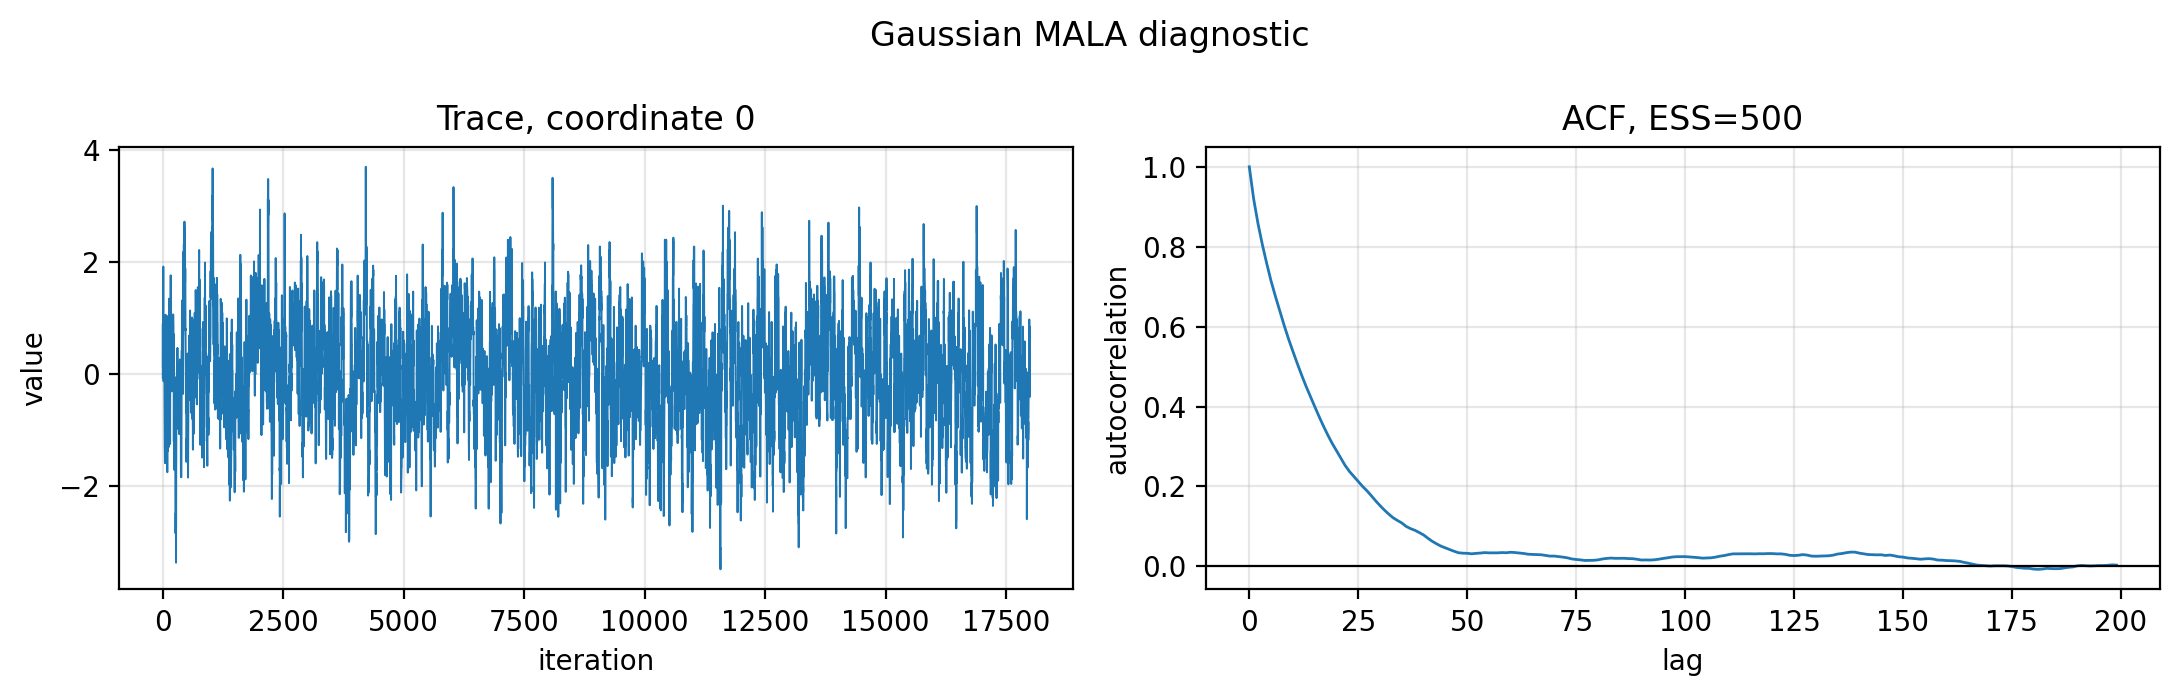
\includegraphics[width=0.9\textwidth]{figures/report/gaussian_trace_acf.png}
\caption{Diagnostics for a single MALA run on the correlated Gaussian
target. \emph{Left:} trace of the first coordinate, showing rapid,
well-mixed exploration with no visible drift. \emph{Right:} the
normalised autocorrelation function of the same coordinate, decaying to
zero within a modest number of lags; the title reports the resulting
effective sample size relative to the chain length.}
\label{fig:gaussian-trace-acf}
\end{figure}

Figure~\ref{fig:gaussian-trace-acf} illustrates the diagnostics on a
single MALA chain: the trace of the first coordinate shows no drift, and
the autocorrelation decays within a few tens of lags, giving an ESS that
is a substantial fraction of the chain length. With the machinery
validated, we turn to the comparison that motivates the rest of the
section.

We run ULA and MALA from the same starting point across a shared
step-size grid. Each run uses $N=12\,000$ iterations and a burn-in of
$2\,000$, and for each $h$ we record the mean error, covariance error,
minimum-coordinate ESS, and MALA acceptance rate. The three diagnostics
are plotted against $h$ in
Figure~\ref{fig:gaussian-comparison}. Read together, they tell a story
that no single panel tells on its own, and it is worth spelling out
because it recurs in every later experiment.

%----------------------------------------------------------------------
% FIGURE 2 — produced by the ULA/MALA step-size sweep cell in M2R.ipynb.
% Three panels: mean error, covariance error, minimum ESS, vs step size.
%----------------------------------------------------------------------
\begin{figure}[ht]
\centering
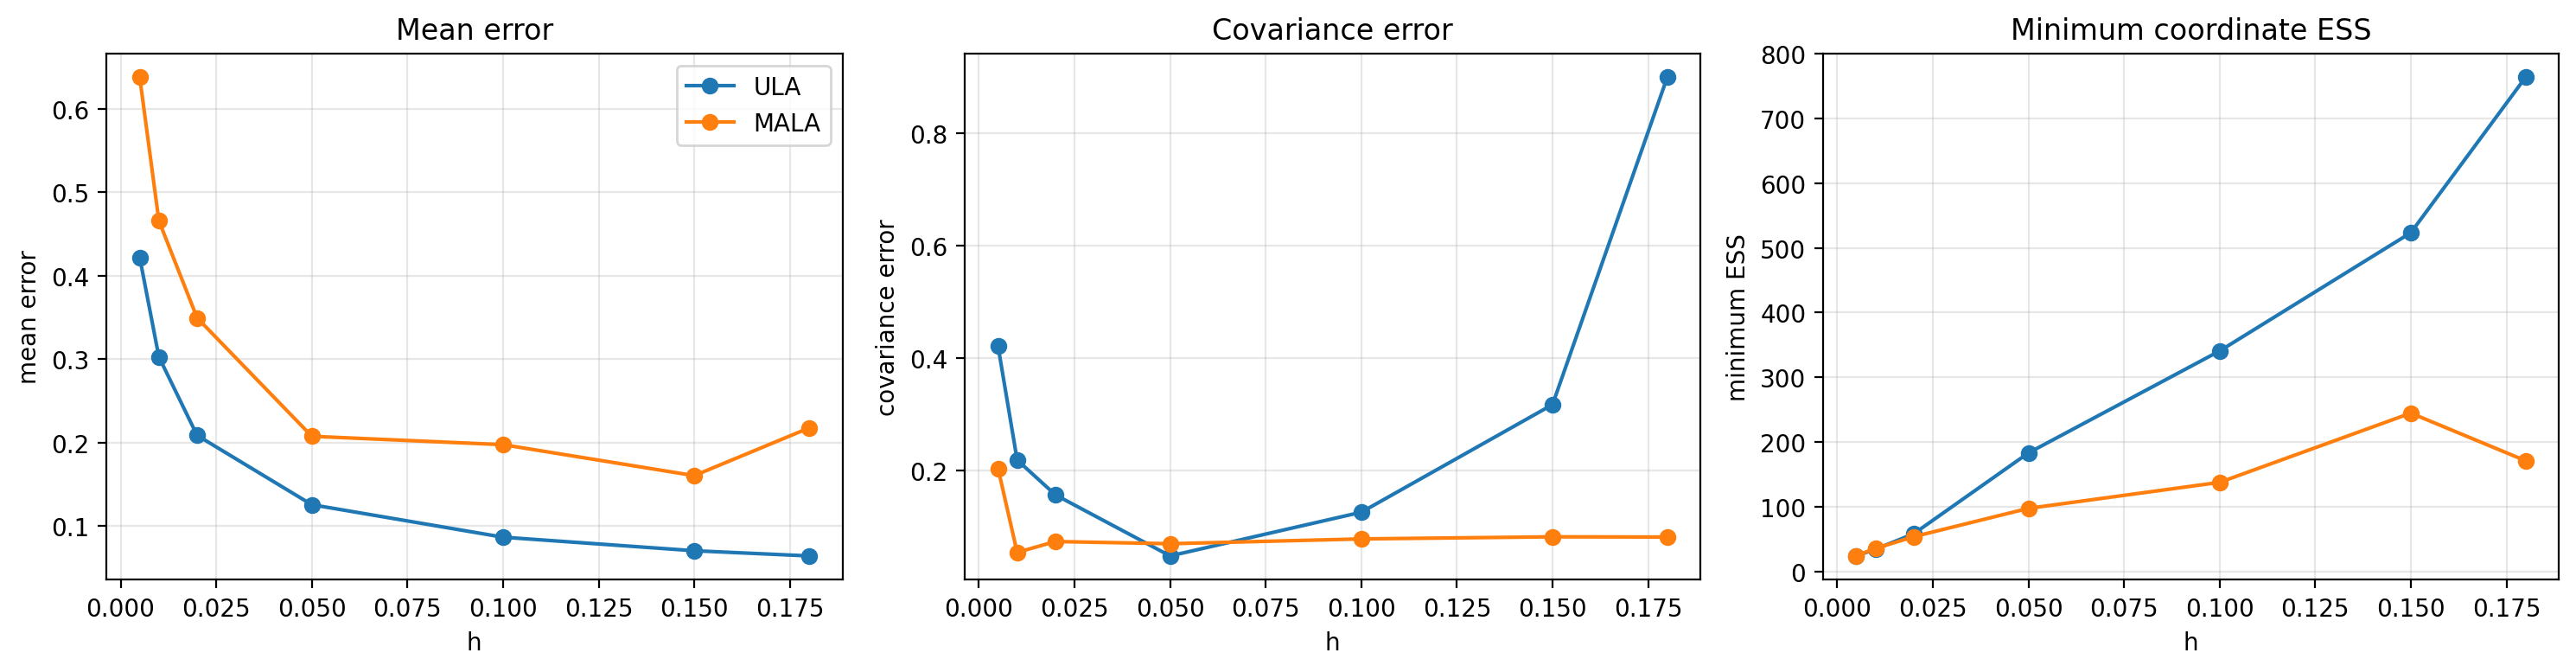
\includegraphics[width=\textwidth]{figures/report/gaussian_ula_mala_sweep.png}
\caption{ULA versus MALA on the correlated Gaussian, as a function of
step size $h$. \emph{Left:} mean error. \emph{Centre:} covariance error
in Frobenius norm. \emph{Right:} minimum-coordinate effective sample size
(higher is better). ULA's covariance error grows with $h$,
exposing its $O(h)$ stationary bias, whereas MALA's stays small; ULA's
ESS climbs monotonically because it never rejects, while MALA's peaks
and then declines as its acceptance rate falls.}
\label{fig:gaussian-comparison}
\end{figure}

Consider the mixing first. ULA never rejects a proposal, so it keeps
moving regardless of the step size, and its ESS rises monotonically as
$h$ grows: larger steps mean larger moves and faster decorrelation. MALA
behaves differently. Its acceptance rate falls steadily as $h$
increases, and each rejection repeats the current state and so injects
positive autocorrelation. The result is that MALA's ESS rises, peaks at
an intermediate step size, and then turns over once rejections dominate.
This non-monotone behaviour is the empirical counterpart of the
well-known optimal scaling of MALA, whose acceptance rate is
asymptotically optimised near $0.574$ \citep{RobertsRosenthal1998}; the
peak in the ESS curve sits in this region.

The mixing panel alone, however, flatters ULA, and this is the central
cautionary point. At the largest step size in the grid, ULA attains both
the lowest mean error and an ESS several times larger than MALA's --- it
appears, on those two diagnostics, to be the better sampler. The
covariance panel corrects the impression. There ULA's error becomes
substantially worse than MALA's at larger step sizes, because ULA is
sampling efficiently from the \emph{wrong} distribution: the Euler
discretisation has shifted its stationary law away from $\pi$ by an
amount that grows with $h$. This is exactly the $O(h)$ covariance bias
derived analytically for the Gaussian case in
Section~\ref{sec:theory-linear-gaussian} and bounded in general by
\citet{Dalalyan2017} and \citet{DurmusMoulines2017}. The reason the bias
hides in the covariance rather than the mean is specific to this target:
the density is centred at the origin, so the first moment is trivial to
estimate and reveals nothing, while the discretisation error distorts
the spread, which is precisely what the covariance panel measures. The
broader lesson, which guides the design of the remaining comparisons, is
that mixing and accuracy must be reported
side by side: a fast chain that mixes well is worthless if it is
converging to the wrong law, and only a diagnostic that is sensitive to
the bias --- here the covariance error --- keeps the comparison honest.

This Gaussian benchmark thus confirms the theory in a controlled setting
and establishes the methodology for what follows. ULA is cheap and mixes
freely but is accurate only at small step sizes; MALA pays for
log-density/proposal work and the occasional rejection but removes the
bias entirely. The next two experiments carry this comparison into
Bayesian linear regression, where the posterior is again Gaussian and
the exact moments remain available, and then into logistic regression,
where the posterior is non-Gaussian and a long reference chain must
stand in for the unavailable truth. The same diagnostics are later
reused for the kinetic sampler of Section~\ref{sec:extension}.

\subsection{Bayesian linear regression}
\label{sec:impl-linear-regression}

The Bayesian linear regression experiment repeats the same comparison in
a slightly higher-dimensional setting where the target remains exactly
tractable. We simulate a regression problem with $d=5$ coefficients and a
Gaussian prior, so the posterior mean and covariance are available in
closed form from Section~\ref{sec:theory-linear-gaussian}. This means
that mean and covariance errors can still be interpreted as errors
against the true posterior rather than against a numerical reference.

The observed behaviour is the same as in the bivariate Gaussian example,
but the larger dimension makes the tuning trade-off more visible. Figure
\ref{fig:linear-cost-aware} shows the main trends. ULA gains
cost-normalised ESS as the step size increases, but the accuracy panels
show the corresponding growth in discretisation error. MALA remains the
most stable on mean and covariance accuracy over the useful part of
the grid, but its efficiency is moderated by the accept--reject step.
KLMC improves as $h$ increases, yet in this linear Gaussian example it
does not clearly dominate MALA on accuracy. The lesson is therefore
unchanged: larger unadjusted steps can decorrelate the chain quickly, but
this is useful only while finite-step bias remains small.

\begin{figure}[ht]
\centering
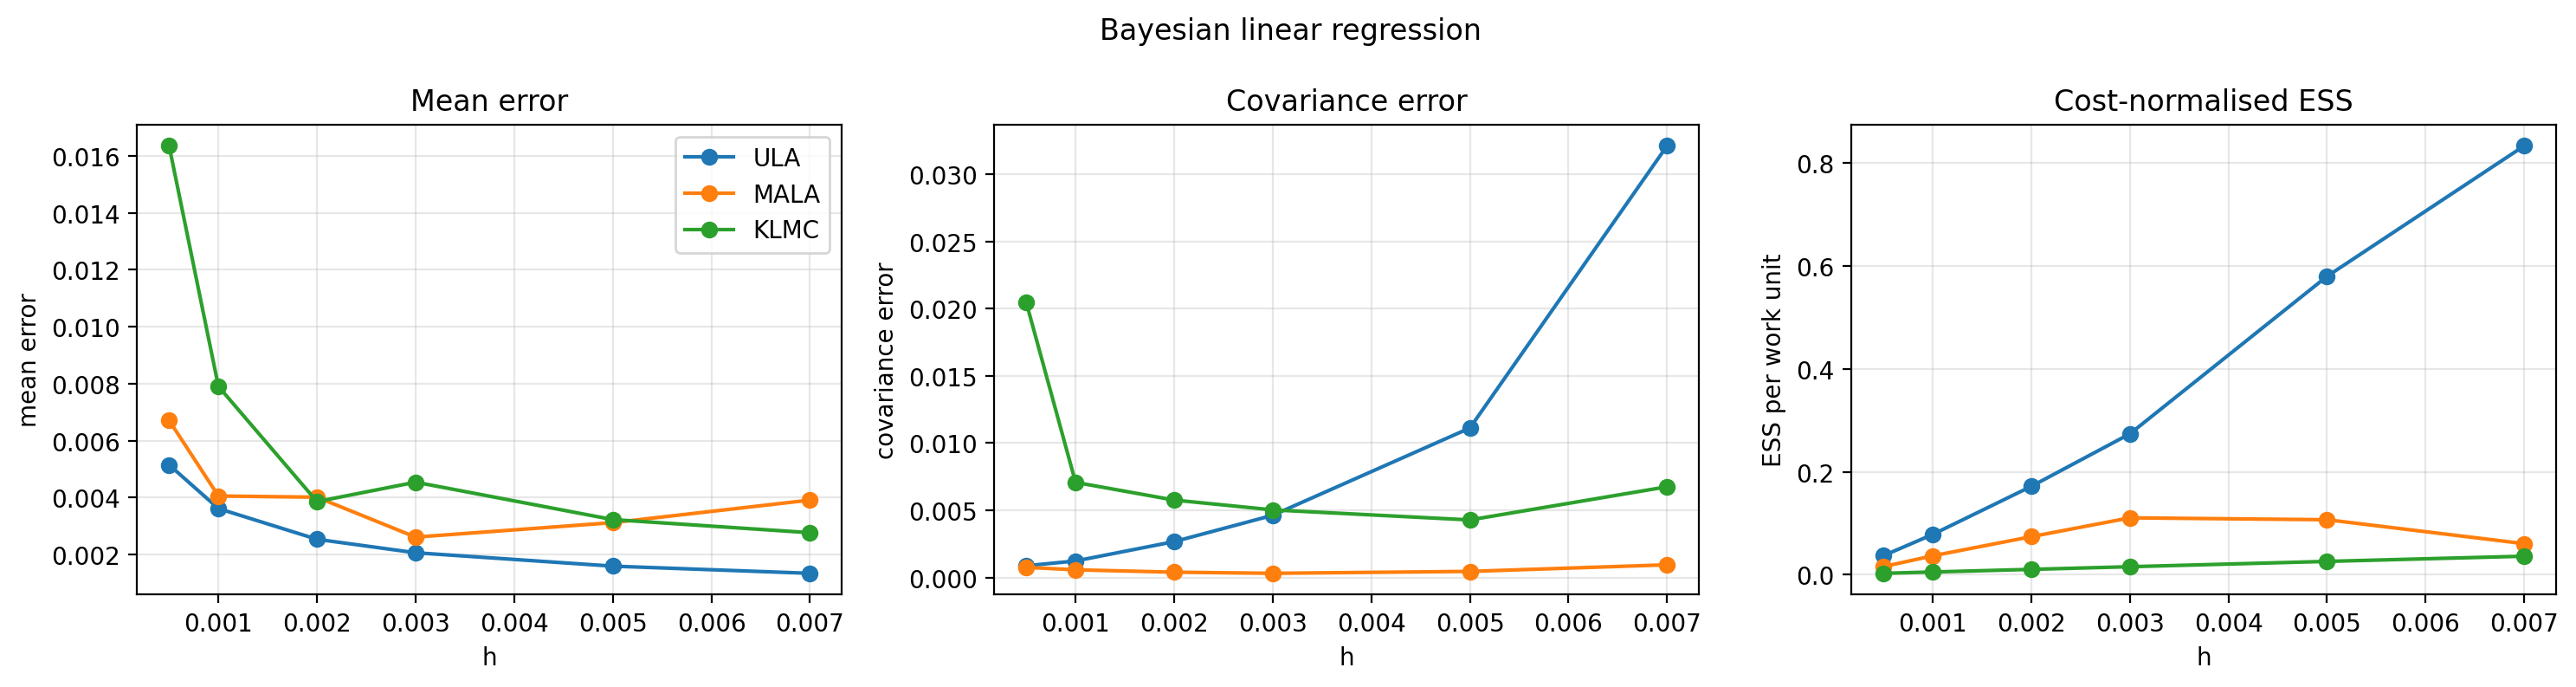
\includegraphics[width=\textwidth]{figures/report/linear_regression_cost_aware.png}
\caption{Cost-aware Bayesian linear regression comparison. The three
panels show mean error, covariance error, and ESS per work unit against
step size.}
\label{fig:linear-cost-aware}
\end{figure}

\subsection{Bayesian logistic regression}
\label{sec:impl-logistic-regression}

Logistic regression removes the convenient Gaussian ground truth. The log
posterior and its gradient are still available, so ULA and MALA can be run
without modification, but exact posterior moments are not. For this
reason, the notebook uses a long small-step MALA chain as a numerical
reference and compares it with a Laplace approximation at the posterior
mode. The two reference summaries are close but not identical: the
Laplace mean differs from the long-run MALA mean by $0.069$, which is a
useful reminder that the logistic posterior is not being treated as
exactly Gaussian.

The shorter ULA, MALA, and KLMC runs are then scored against this
numerical reference, not against an analytic truth. Figure
\ref{fig:logistic-cost-aware} shows that the same relationships persist
in the non-Gaussian model. ULA again becomes increasingly efficient in
ESS per work unit as the step size grows, but this is matched by
worsening mean and covariance error. MALA is more stable on the
accuracy diagnostics because the Metropolis correction controls the
finite-step bias. KLMC is competitive for a well-tuned step size, but its
accuracy is also step-size dependent because the implementation is
unadjusted. This is the practical version of the theoretical trade-off:
ESS is informative only when read together with accuracy and cost.

\begin{figure}[ht]
\centering
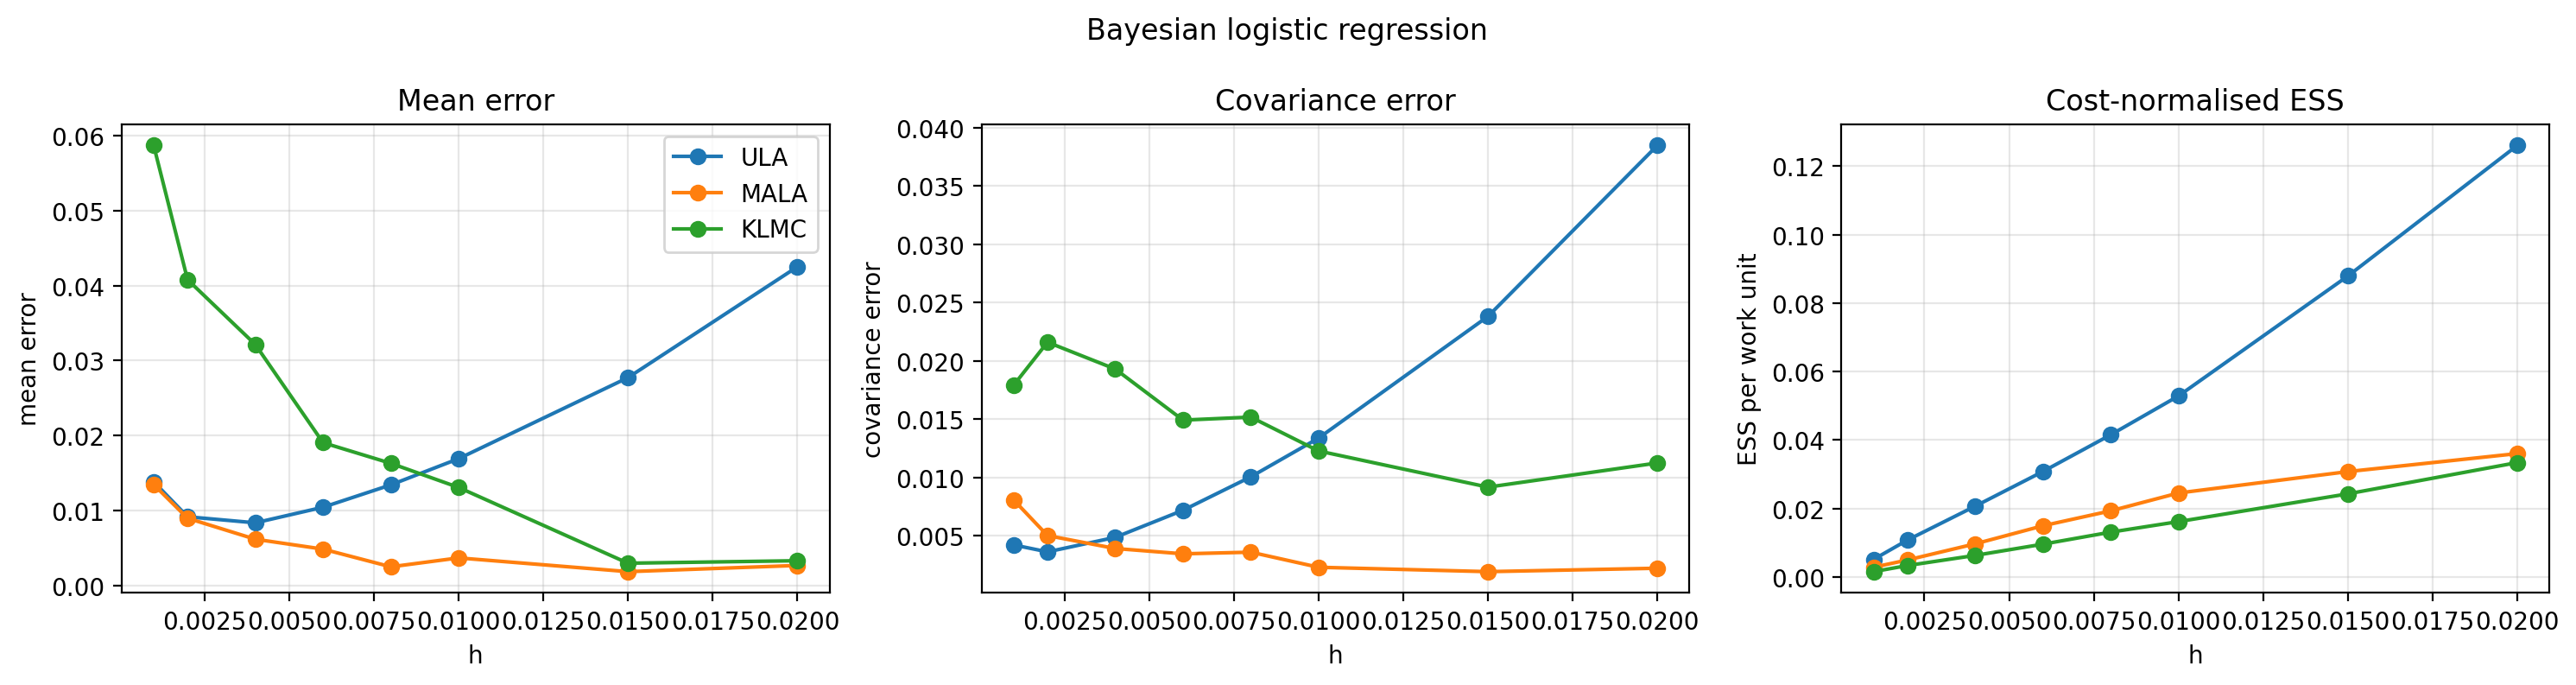
\includegraphics[width=\textwidth]{figures/report/logistic_regression_cost_aware.png}
\caption{Cost-aware Bayesian logistic regression comparison against the
long MALA reference chain. The three panels show mean error, covariance
error, and ESS per work unit against step size.}
\label{fig:logistic-cost-aware}
\end{figure}

%%%%%%%%%%%%%%%%%%%%%%%%%%%%%%%%%%%%%

\subsection{Kinetic Langevin cost-aware experiments}
\label{sec:ext-experiments}

The notebook compares ULA, MALA, and KLMC on the correlated Gaussian
using the same post-burn-in diagnostics as before, together with ESS per
work unit.
The friction parameter is fixed at $\gamma=2.0$ for this comparison. The
point is not to identify a single global optimum in the grid, but to
compare the same accuracy--mixing trade-off across the three algorithms.

The comparison reinforces the earlier warning about ESS. ULA can obtain a high
ESS per work unit because it never rejects and uses only one gradient per
step, but its covariance error remains visibly affected by finite-step
bias. MALA is the most accurate method in this grid on the moment-error
diagnostics, but this comes at the cost of extra target work and
rejections. KLMC sits between these two
behaviours in the tested regime: it is approximate like ULA and requires
tuning of both $h$ and $\gamma$, but the momentum variable can improve
cost-aware mixing at larger step sizes.

\subsection{Beyond the Strongly Log-Concave Setting [NOT SURE YET]}
\label{sec:ext-nonconvex}

The theory quoted above is stated for smooth strongly log-concave targets.
The logistic regression experiment is still convex under Gaussian
regularisation, but it is no longer an exactly Gaussian benchmark. We
therefore avoid extending the theoretical guarantees beyond their stated
setting. The non-Gaussian experiment is used only as an empirical check
that the same diagnostics--accuracy against a reference, ESS, acceptance
rate, and work-normalised cost--remain informative when exact posterior moments
are unavailable. Figure~\ref{fig:logistic-cost-aware} shows that this
diagnostic set is still useful: ULA's cost-normalised ESS rises with $h$
while its moment errors worsen, MALA remains stable on covariance error,
and KLMC can be competitive for a well-tuned step size without a
Metropolis correction.

\subsection{KLMC interpretation}
\label{sec:results-klmc-interpretation}

The KLMC results should therefore be read as a proof of concept rather
than as a universal ranking. The theoretical bounds suggest that kinetic
dynamics can improve some dimension and precision dependences under
specific metrics and assumptions, but this is not a like-for-like
dominance statement over the overdamped algorithms. In practice, the
observed behaviour depends on the target, the implemented integrator, and
the friction parameter. The choice
$\gamma\asymp\sqrt{m+M}$ should therefore be read as a theorem-specific
tuning rule rather than a universal optimum. Second-order KLMC methods
use Hessian information and can further improve the precision dependence
\citep[Section~4]{DalalyanRiouDurand2020}, but these are not implemented
here.

%%%%%%%%%%%%%%%%%%%%%%%%%%%%%%%%%%%%%

The common pattern across the experiments is that raw mixing and accuracy need not move together. ULA can obtain large ESS, especially at larger step sizes, but its mean and covariance errors reveal the finite-step bias. MALA controls this bias through the Metropolis correction, at the cost of rejections and a more expensive transition. KLMC provides a third trade-off: it uses momentum and one gradient step per iteration in the implemented scheme, but it remains unadjusted and is sensitive to step size and friction.

\section{Discussion}

\begin{center}
\textbf{Qualitative summary of the three Langevin-based methods}

\centering
\small
\begin{tabular}{p{0.11\textwidth}p{0.22\textwidth}p{0.19\textwidth}p{0.18\textwidth}p{0.15\textwidth}}
\toprule
Method & Interpretation & Accuracy & Mixing and cost & Main weakness \\
\midrule
ULA & Direct Euler discretisation of overdamped Langevin diffusion. &
Biased for finite $h$; exact only as $h\to0$ in the limit. &
One gradient per step; can have high raw ESS at large $h$. &
Large steps can sample efficiently from the wrong law. \\
MALA & ULA proposal plus Metropolis--Hastings correction. &
Targets $\pi$ exactly asymptotically, after adequate mixing. &
Extra target/proposal work per step; ESS depends on acceptance rate. &
Poor tuning causes many rejections and slower exploration. \\
KLMC & Underdamped dynamics on position and velocity. &
Integrator-dependent in the unadjusted implementation. &
Momentum can improve cost-aware mixing. &
Requires tuning $h$ and $\gamma$; theory depends on conditioning. \\
\bottomrule
\end{tabular}
\end{center}

The main interpretation is that the three algorithms should not be ranked by a single number. ULA is the simplest and cheapest discretisation, so it is attractive when a small amount of bias is acceptable or when the step size can be chosen conservatively. MALA uses the same local Langevin proposal but corrects it with a Metropolis--Hastings step, making it more reliable for exact targeting at the price of rejections and additional target/proposal computations. KLMC changes the underlying dynamics by adding momentum; this can improve exploration, but the unadjusted implementation is still sensitive to the integrator, the step size, and the friction parameter.

There are several caveats to the numerical comparisons. First, the ESS reported here is the minimum coordinate-wise ESS, not a multivariate ESS, and values near the post-burn-in chain length should be read as diagnostic summaries rather than exact independent sample counts. Second, the cost normalisation uses the simple work count $C=N_{\nabla}+N_{\log\pi}$ rather than wall-clock time. This charges MALA for the log-density work needed by the accept--reject correction, but it still ignores proposal-density arithmetic, linear algebra constants, vectorisation, and implementation-level timing effects. Third, the logistic-regression errors are distances to a long MALA reference chain rather than exact posterior errors; no multi-chain convergence or Monte Carlo standard error analysis is included. Finally, KLMC is unadjusted in these experiments, so high ESS can still correspond to efficient exploration of a biased discretisation.

\section{Conclusion}

This project studies Langevin-based MCMC as a practical approximation to
an ideal continuous-time diffusion. The continuous-time overdamped
Langevin process has the target distribution as its invariant law, but it
cannot usually be simulated exactly. Discretisation makes simulation
possible and leads to ULA, but it also introduces finite-step bias. MALA
responds by adding a Metropolis correction to the same proposal, removing
the asymptotic bias at the cost of rejections and additional gradient
work. KLMC responds differently by augmenting the dynamics with momentum,
which can improve exploration but introduces a friction parameter and a
more complex discretisation.

The experiments confirm that the best sampler is not simply the one with
the highest ESS. Efficient sampling requires accurate estimation after
burn-in at reasonable computational cost. ULA, MALA, and KLMC each
navigate this trade-off differently, so the right comparison must report
accuracy, burn-in and mixing diagnostics, acceptance behaviour where
relevant, and cost per effective sample.

%%%%%%%%%%%%%%%%%%%%%%%%%%%%%%%%%%%%%

% ADD TO .bib the following two entries:

% @article{RobertsTweedie1996,
%   author  = {Roberts, Gareth O. and Tweedie, Richard L.},
%   title   = {Exponential convergence of {Langevin} distributions and their discrete approximations},
%   journal = {Bernoulli},
%   volume  = {2}, number = {4}, pages = {341--363}, year = {1996}}

% @misc{Duncan2016,
%   author       = {Duncan, A.},
%   title        = {{M4A44}: Computational Stochastic Processes},
%   year         = {2016},
%   howpublished = {Lecture notes, Imperial College London}}


%%%%%%%%%%%%%%%%%%%%%%%%%%%%%%%%%%%%%

%%%%%%%%%%%%%%%%%%%%%%%%%%%%%%%%%%%%%
\bibliography{bibliography.bib}
%%%%%%%%%%%%%%%%%%%%%%%%%%%%%%%%%%%%%

\end{document}
